\documentclass[12pt, a4paper, fontset=fandol]{ctexart}
\ctexset{
    section = {
        format = \Large\bfseries\raggedright
    }
}

\usepackage{geometry} 
\usepackage{graphicx} 
\usepackage{listings} 
\usepackage{xcolor}   
\usepackage{float}    
\usepackage{fancyhdr}
\pagestyle{fancy}     
\fancyhf{}            
\usepackage{amsmath}
\renewcommand{\headrulewidth}{0pt} 
\cfoot{\thepage}      

\geometry{left=2.5cm, right=2.5cm, top=2.5cm, bottom=2.5cm}
\definecolor{lightgray}{gray}{0.95}

\lstset{
    basicstyle=\ttfamily\small,        % 基本字体样式
    keywordstyle=\color{blue}\bfseries,% 关键字颜色
    commentstyle=\color{green!50!black},% 注释颜色
    stringstyle=\color{red},           % 字符串颜色
    showstringspaces=false,            % 不显示字符串内的空格
    numbers=left,                      % 行号在左侧
    numberstyle=\tiny\color{gray},     % 行号字体设置
    frame=single,                      % 给代码加边框
    breaklines=true,                   % 自动折行
    tabsize=4,                         % Tab键宽度
    backgroundcolor=\color{lightgray}
}

% ========== 代码块格式设置 ==========
\usepackage{tcolorbox}
\tcbuselibrary{listings, breakable} % 如果用 listings，改成 \tcbuselibrary{listings}

\newtcblisting{mycode}[2][]{%
    listing only,
    breakable,
    colback=gray!5, % 背景色
    colframe=gray!40, % 边框色
    arc=3mm, % 圆角大小
    boxrule=0.5pt,
    listing options={language=#2, basicstyle=\ttfamily\small, breaklines, numbers=none, frame=none},
    #1
}
\usepackage{listings}


\usepackage[hidelinks]{hyperref}
\graphicspath{{figures/}}
\setcounter{tocdepth}{2}
\begin{document}
\begin{center}
    \Huge{自然语言处理作业一} \\[0.5cm]
    \Large{文本分类实验报告} \\[0.5cm]
    \normalsize
    姓名：\underline{王策} \quad 学号：\underline{2410966}\\[0.2cm]
\end{center}
\vspace{0.5cm}
{\small\linespread{1}\selectfont\tableofcontents}
\clearpage

\section{实验目的}
本次作业要求使用不同的文本表示方法，对 NYT 新闻进行分类。新闻分为 business、politics 和 sports 三类。三个任务使用同一份训练集、验证集和测试集，最后比较 Accuracy 和 Macro-F1。

Task 1 使用 Binary Bag of Words 和 Word Frequency，将文章转换成词袋向量，再训练逻辑回归。Task 2 分别使用 GloVe、AG News 训练的 Word2Vec 和 NYT 训练的 Word2Vec，把每篇文章表示为 100 维平均词向量，再训练逻辑回归。Task 3 使用 BERT-base-uncased，设置最大长度 64，微调 3 轮。

\section{数据处理}
NYT 共有 11,519 篇新闻，每行包含 text 和 label。AG News 有 90,000 篇文本，只用于训练词向量，没有类别标签。NYT 的类别数量为：business 1429 篇、politics 1451 篇、sports 8639 篇。

按照 8:1:1 划分 NYT。各任务调用同一个 \texttt{load\_data()}先取出 20\% 的数据，再将这部分等分为验证集和测试集；两次划分都按标签分层，使三个集合的类别比例接近。
\begin{table}[H]\centering
\begin{tabular}{lrrrr}\hline\hline
数据 & 总数 & business & politics & sports\\\hline
训练集 & 9215 & 1143 & 1161 & 6911\\
验证集 & 1152 & 143 & 145 & 864\\
测试集 & 1152 & 143 & 145 & 864\\\hline\hline
\end{tabular}
\caption{本实验实际使用的数据划分。}
\end{table}

\subsection{文本处理与评价指标}
词袋使用 \texttt{CountVectorizer} 的默认分词规则：转为小写，提取至少两个字符的词元。词向量使用小写正则 \texttt{[a-z]+}，只保留英文片段。BERT 使用模型配套的 WordPiece 分词器。它们的分词规则不同，报告比较的是这些具体实现的结果。

准确率计算公式：
\begin{equation}
\mathrm{Accuracy}=\frac{\text{正确预测数}}{\text{测试样本总数}}.
\end{equation}
Macro-F1计算公式：
\begin{equation}
P=\frac{TP}{TP+FP},\quad R=\frac{TP}{TP+FN},\quad
F1=\frac{2PR}{P+R},\qquad \mathrm{Macro\mbox{-}F1}=\frac{F1_1+F1_2+F1_3}{3}.
\end{equation}

\section{Task 1：Bag of Words}
\subsection{原理}
词袋模型先在训练文本中建立词表，给每个词分配一个固定位置。之后，每篇文章都变成与词表等长的向量。Binary 只记录某个词有没有出现；Word Frequency 记录它出现了多少次。

得到向量后使用逻辑回归分类。模型为各类别学习一组词权重，将输入向量与权重相乘并加上偏置，得到类别得分。多分类时通过 softmax 将得分转换为概率，选择概率最大的类别。

\subsection{代码实现}
在 \texttt{task1.py} 中，两种方法只需要设置不同的向量器：
\begin{mycode}{python}
methods = [
    ('bow_binary', CountVectorizer(binary=True)),
    ('bow_count', CountVectorizer()),
]
\end{mycode}
\texttt{binary=True} 把非零词频都改为 1。默认情况下不设置这个参数，就是保留出现次数。两个方法都只在训练集建立词表：
\begin{mycode}{python}
features = {'train': vectorizer.fit_transform(parts['train'].text)}
for split in ['val', 'test']:
    features[split] = vectorizer.transform(parts[split].text)
\end{mycode}
\texttt{fit\_transform} 包含学习词表和转换文本两个动作；\texttt{transform} 只按已有词表转换。验证集和测试集不 fit。本次训练词表大小为 60,980，训练矩阵形状为 $9215\times60980$。

\texttt{common.py} 的 \texttt{fit\_lr} 负责训练逻辑回归。从 $C=0.1,1,10$ 中选择验证 Macro-F1 最高的模型；最大迭代次数为 1500，容差为 0.001。$C$ 越小，正则约束越强，模型不容易给个别词过大的权重。选完参数后，再用固定模型预测测试集。

\subsection{实验结果}
\begin{table}[H]\centering
\begin{tabular}{lrrrr}\hline\hline
方法 & 验证 F1：$C=0.1$ & $C=1$ & $C=10$ & 选择的 $C$\\\hline
Binary & 96.20 & 95.84 & 95.38 & 0.1\\
词频 & 96.45 & 96.22 & 95.38 & 0.1\\\hline\hline
\end{tabular}
\caption{Task 1 验证集选参结果，F1 单位为百分数。}
\end{table}
\begin{table}[H]\centering
\begin{tabular}{lrrr}\hline\hline
方法 & 测试 Accuracy & 测试 Macro-F1 & 错误篇数\\\hline
Binary & 98.87\% & 97.18\% & 13\\
词频 & 99.05\% & 97.65\% & 11\\\hline\hline
\end{tabular}
\caption{Task 1 的测试结果。}
\end{table}
词频的两个指标都略高于 Binary，但净多判对的只有 2 篇。进一步比较逐篇结果：Binary 独自判对 4 篇，词频独自判对 6 篇，两者共同判错 7 篇。因此不是词频在每一篇新闻上都更好。
\begin{figure}[H]\centering
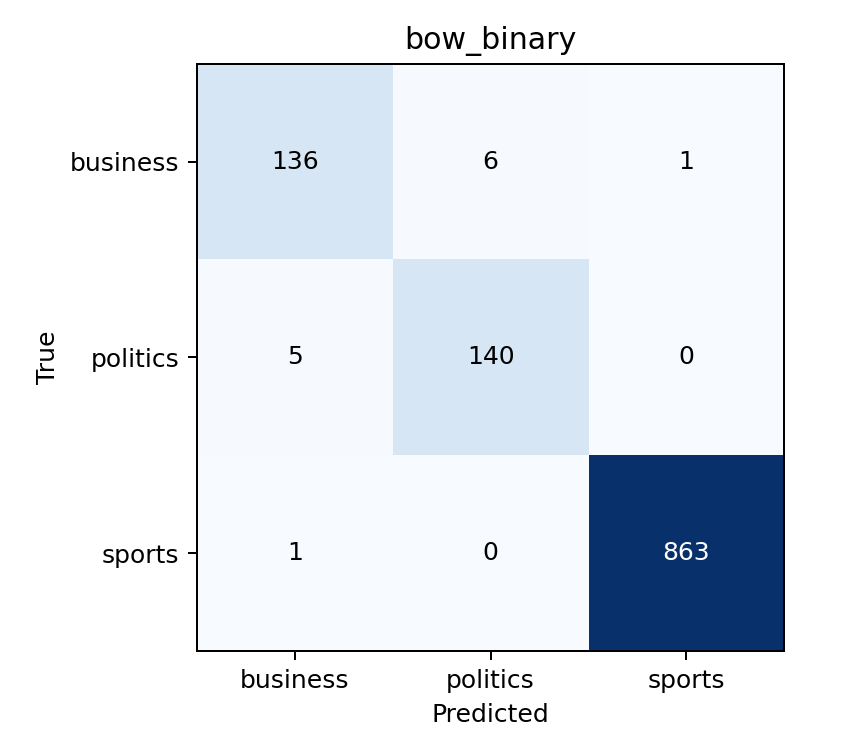
\includegraphics[width=.48\linewidth]{bow_binary_confusion.png}\hfill
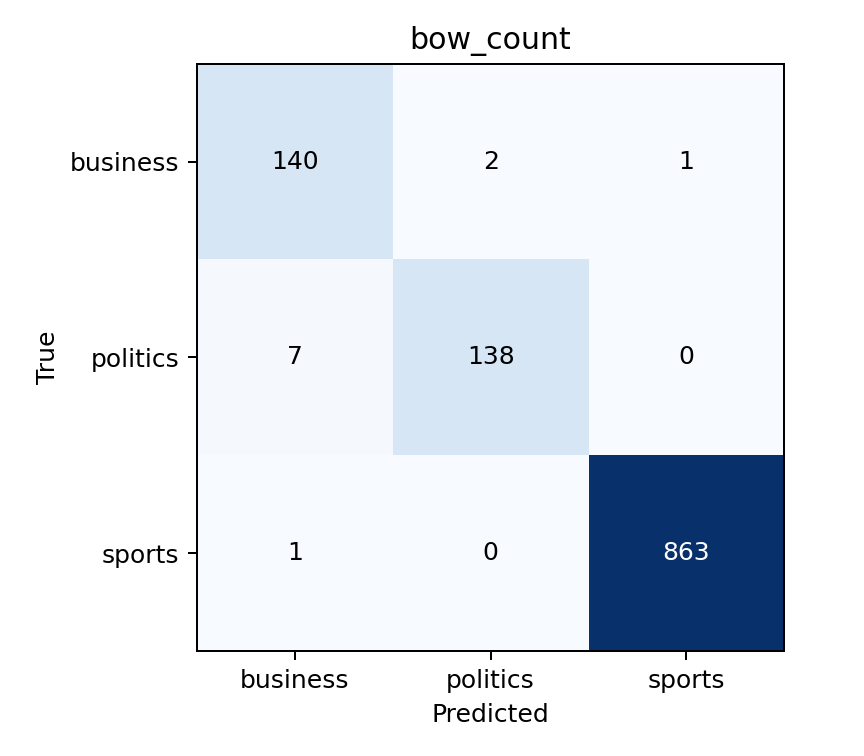
\includegraphics[width=.48\linewidth]{bow_count_confusion.png}
\caption{Binary 与词频的混淆矩阵。行是真实类别，列是预测类别。}
\end{figure}
两个模型都能较好地区分体育新闻，错误主要发生在 business 与 politics 之间。词频把 7 篇政治新闻预测为商业，而 Binary 对应为 5 篇；此外，词频把商业预测为政治的错误从 6 篇降到了 2 篇。说明总体提高也可能使某一类错误增加。

以词频的 business 类为例，143 篇中分对 140 篇；同时有 7 篇 politics 和 1 篇 sports 被误判为 business。因此它的 Precision 为 $140/148=94.59\%$，Recall 为 $140/143=97.90\%$，F1 为 96.22\%。

\section{Task 2：Word Embedding}
\subsection{用平均词向量表示文章}
词袋每一维对应一个词，而词向量用一组较短的实数表示一个词。具有相似用法的词，向量可能比较接近。本次实验使用 100 维词向量。

一篇文章包含多个词，需要先把词向量合并成一个文档向量。采用平均方法：
\begin{equation}
\boldsymbol{e}(d)=\frac{1}{n}\sum_{i=1}^{n}\boldsymbol{e}(w_i),
\end{equation}
其中 $n$ 是能够查到向量的词的数量。重复词按出现次数参与平均，查不到向量的词跳过。若没有任何有效词，返回 100 维零向量；


\subsection{GloVe 预训练词向量}
GloVe 根据大规模语料中的词共现关系学习词向量。本次直接使用 Stanford 的 \texttt{glove.6B.100d}。文件每行是一个词及其 100 个数。

词向量分词函数如下：
\begin{mycode}{python}
def tokenize(text):
    return re.findall(r'[a-z]+', text.lower())
\end{mycode}
\texttt{lower()} 将英文转为小写；\texttt{[a-z]+} 表示连续的一个或多个英文字母。这样可以减少大小写造成的词形差异，但数字、标点不进入向量平均。有些缩写会被拆开，这是当前分词方式的一个局限。

读取 GloVe 后，按词查表并平均：
\begin{mycode}{python}
words = tokenize(text)
valid = [vectors[word] for word in words if word in vectors]
if valid:
    rows.append(np.mean(valid, axis=0))
else:
    rows.append(np.zeros(100, dtype=np.float32))
\end{mycode}
\texttt{valid} 是多个 100 维向量组成的列表。\texttt{axis=0} 表示沿词的方向求平均，得到一个 100 维文档向量。之后仍然调用与 Task 1 相同的逻辑回归训练函数。

\subsection{在 AG News 和 NYT 上训练 Word2Vec}
Word2Vec 通过词的上下文学习向量。本次使用 skip-gram，即根据中心词学习它附近词的关系。它不需要分类标签，因此 AG News 只有文本也可以用于训练。

两种训练数据分别为全部 AG News 文本和 NYT 的训练部分。代码使用相同参数：
\begin{mycode}{python}
model = Word2Vec(
    sentences=sentences, vector_size=100,
    window=5, min_count=2,
    workers=1, sg=1, epochs=5, seed=42,
)
vectors = model.wv
\end{mycode}
\begin{table}[H]\centering
\begin{tabular}{llp{8cm}}\hline\hline
参数 & 设置 & 含义\\\hline
vector\_size & 100 & 每个词用 100 个数表示\\
sg & 1 & 使用 skip-gram\\
window & 5 & 上下文窗口上限\\
min\_count & 2 & 忽略只出现一次的词\\
epochs & 5 & 词向量训练 5 轮\\
workers & 1 & 单线程，减少随机变化\\
seed & 42 & 固定随机种子\\\hline\hline
\end{tabular}
\caption{两组 Word2Vec 共用的参数。}
\end{table}
代码中的 \texttt{sentences} 是由各篇文章的分词列表组成的列表，没有另外按句子切分。\texttt{model.wv} 用来按词取向量。获得词向量后，AG 和 NYT 两个版本都对同一份 NYT 训练、验证和测试数据求平均，并在 NYT 训练标签上拟合逻辑回归。

\subsection{实验结果}
三种文档向量都为 100 维，逻辑回归仍在 $C=0.1,1,10$ 中按验证 Macro-F1 选择。GloVe 和 NYT Word2Vec 选择 $C=10$，AG Word2Vec 选择 $C=1$。
\begin{table}[H]\centering
\begin{tabular}{lrrrr}\hline\hline
方法 & 验证 Macro-F1 & 测试 Accuracy & 测试 Macro-F1 & 错误篇数\\\hline
GloVe & 95.10\% & 98.35\% & 96.19\% & 19\\
AG Word2Vec & 91.14\% & 97.14\% & 93.07\% & 33\\
NYT Word2Vec & 93.90\% & 98.00\% & 95.06\% & 23\\\hline\hline
\end{tabular}
\caption{Task 2 的结果。}
\end{table}
\begin{table}[H]\centering
\begin{tabular}{lrrr}\hline\hline
方法 & business F1 & politics F1 & sports F1\\\hline
GloVe & 94.52\% & 94.41\% & 99.65\%\\
AG Word2Vec & 89.86\% & 89.75\% & 99.59\%\\
NYT Word2Vec & 92.41\% & 93.01\% & 99.77\%\\\hline\hline
\end{tabular}
\caption{三种词向量在不同类别上的表现。}
\end{table}
GloVe 在三组中总体最好，NYT Word2Vec 高于 AG Word2Vec。三种方法在 sports 上都比较好，主要差距出现在 business 和 politics。可见只看总体 Accuracy，会不容易注意到两个小类别的差异。
\begin{figure}[H]\centering
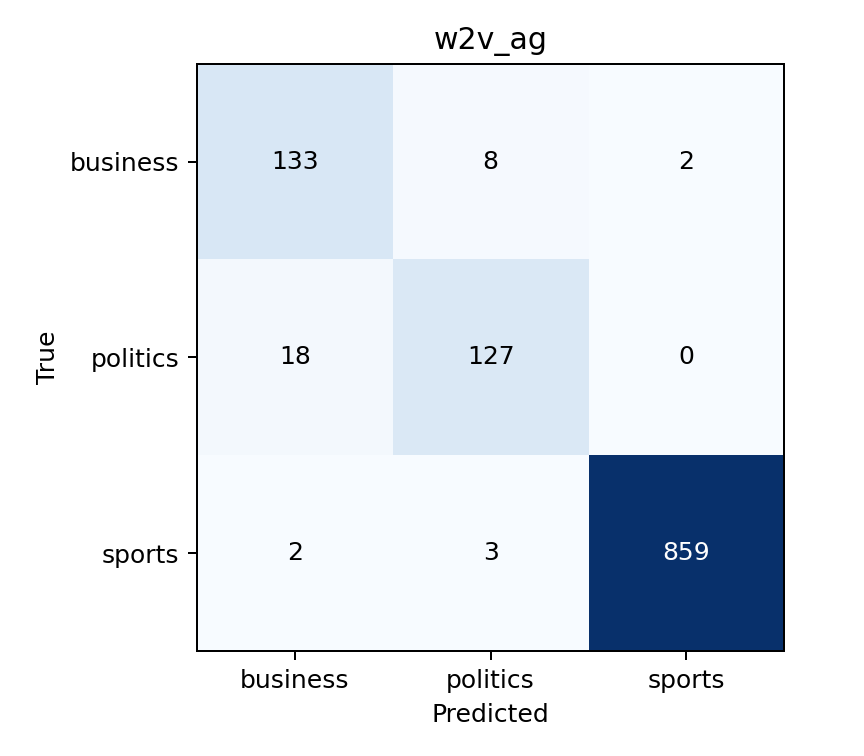
\includegraphics[width=.48\linewidth]{w2v_ag_confusion.png}\hfill
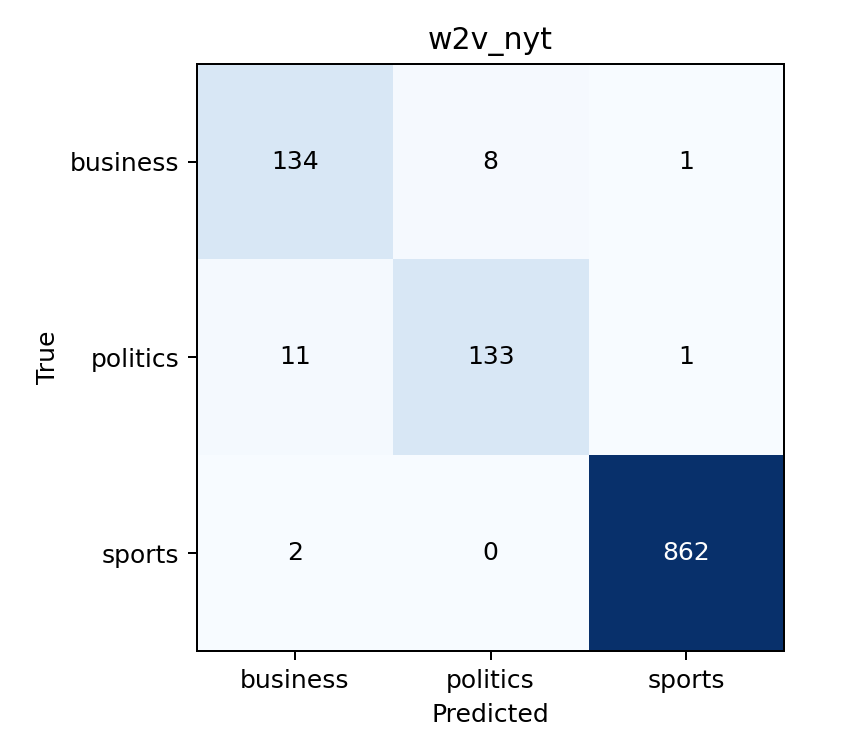
\includegraphics[width=.48\linewidth]{w2v_nyt_confusion.png}
\caption{AG 与 NYT Word2Vec 的混淆矩阵。}
\end{figure}
AG 把 18 篇 politics 分成 business，NYT 对应为 11 篇。NYT 的政治类 Recall 从 AG 的 $127/145$ 提高到 $133/145$。两者把 business 分成 politics 的数量都是 8 篇，因此可以发现提高并不是所有方向都一致发生的。

\subsection{覆盖率分析}
程序在求平均时统计总词数和能够查到向量的词数，两者之比就是 token 覆盖率。重复词按出现次数计数。
\begin{table}[H]\centering\small
\begin{tabular}{lrrr}\hline\hline
来源 & 本地训练文章数 & 本地训练 token 数 & 测试覆盖率\\\hline
GloVe & 使用公开预训练向量 & 不在本地训练 & 99.79\%\\
AG Word2Vec & 90,000 & 3,454,568 & 97.35\%\\
NYT Word2Vec & 9,215 & 5,985,752 & 99.29\%\\\hline\hline
\end{tabular}
\caption{两种本地语料的规模，以及三种向量的测试覆盖率。}
\end{table}
AG 虽然文章数更多，但文章较短，按当前分词方式得到的 token 总数反而少于 NYT 训练集。NYT 与测试新闻来自同一数据集，主题更接近，这可能有助于它学习适合本任务的向量。GloVe 使用外部大规模预训练，测试覆盖率也最高，这些因素可能有助于它取得较好的结果。

三种平均词向量都没有超过 Task 1 的词频模型。我理解一个原因是：词袋可以直接保留一个很有区分力的词，而平均词向量把整篇新闻压缩成 100 个数，少量关键词可能被其它内容冲淡。平均还丢失词序，无法区分同一个词在不同上下文里的意义。

\subsection{扩展实验：训练数据量对分类效果的影响}
前面的实验使用全部训练数据。这里进一步比较：如果能够用于分类训练的新闻变少，词频和 GloVe 平均词向量的效果会怎样变化？两种表示都使用逻辑回归，主要区别在于词频需要从当前训练文本建立词表，而 GloVe 已经包含外部语料中学到的词向量。

保持原来的验证集和测试集不变，只在 9215 篇训练新闻中按类别比例抽取 10\%、25\%、50\% 和 100\%。前三种比例分别使用随机种子 42、43、44 抽样，每次两种方法使用完全相同的训练子集。各比例独立抽样，不要求小子集包含在大子集中。100\% 时没有抽样变化，因此只运行一次，不将同一个结果视为三次独立重复。

词频模型每次只在当前训练子集建立词表，验证和测试文本使用该词表转换。GloVe 始终使用同一份公开的 100 维向量，按原方法对全文求平均；它没有在这些新闻上重新训练词向量。两种方法分别按固定验证集的 Macro-F1，从 $C=0.1,1,10$ 中选择参数，测试集只用于最终评价。因此，本实验比较的是同样数量的本地标注数据下两种方法的表现，并不是两者预先接触过的全部文本数量相同。

\begin{table}[H]\centering
\begin{tabular}{rrrr}\hline\hline
训练比例 & 训练篇数 & 词频 Macro-F1 & GloVe Macro-F1\\\hline
10\% & 921 & $95.33\pm0.74$ & $95.92\pm1.43$\\
25\% & 2303 & $96.39\pm0.35$ & $95.30\pm0.86$\\
50\% & 4607 & $96.70\pm0.32$ & $94.74\pm0.14$\\
100\% & 9215 & $97.65$ & $96.19$\\\hline\hline
\end{tabular}
\caption{不同训练数据量下的测试 Macro-F1，单位为百分数。前三行是三次抽样的均值与样本标准差，最后一行是全量训练的单次结果。}
\end{table}
\begin{figure}[H]\centering
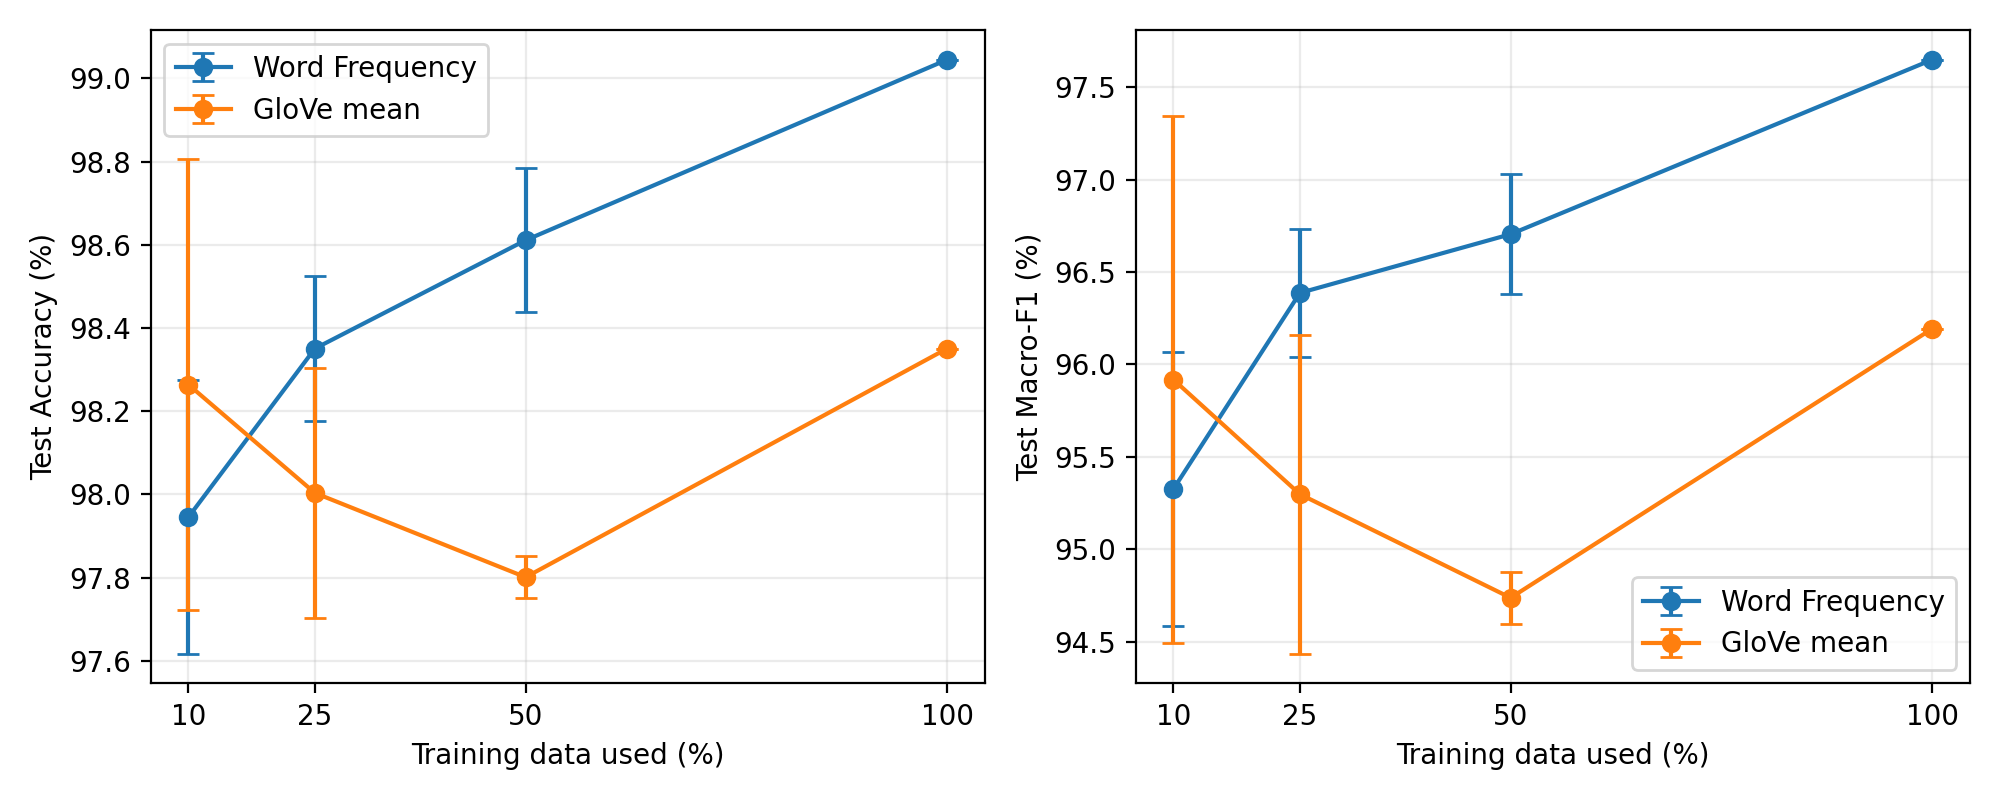
\includegraphics[width=.98\linewidth]{training_size.png}
\caption{训练数据量与测试成绩}
\end{figure}

从结果看，词频的平均 Macro-F1 随训练数据量增加，从 95.33\% 提升到 97.65\%，提高约 2.32 个百分点。10\% 时的抽样标准差为 0.74 个百分点，到 50\% 时降为 0.32 个百分点，说明在本次抽样中，更多训练新闻既提高了平均成绩，也减小了不同子集之间的波动。增加训练数据可能使模型见到更多词汇及其与类别的联系，因而能更好地区分测试新闻。

只有 10\% 训练数据时，GloVe 的平均 Macro-F1 比词频高约 0.59 个百分点，说明已有的预训练表示在少量标注数据下可能有所帮助。不过，GloVe 三次的成绩约为 97.02\%、96.42\% 和 94.31\%，波动较大，而且并非每次都高于词频，因此不能据此认定 GloVe 在小样本情况下稳定更好。

\section{Task 3：BERT 微调}
\subsection{参数设置}
前两个任务先固定文本表示，再训练逻辑回归。BERT 则先将文本切成 WordPiece 子词，通过编码器得到与上下文有关的表示，再接分类层。在本任务中，分类层和 BERT 编码器一起更新，即微调。

使用模型 \texttt{google-bert/bert-base-uncased}。代码中的最大长度为 64，训练 3 轮。BERT 的 64 个位置包含 \texttt{[CLS]} 和 \texttt{[SEP]}，因此单篇新闻最多输入 62 个正文 WordPiece。
\begin{table}[H]\centering
\begin{tabular}{ll}\hline\hline
参数 & 设置\\\hline
预训练模型 & BERT-base-uncased\\
最大序列长度 & 64\\
训练轮数 & 3\\
批大小 & 16\\
优化器 & AdamW\\
学习率 & $2\times10^{-5}$\\
权重衰减 & 0.01\\
学习率安排 & 前 10\% 步数预热，然后线性下降\\
模型选择 & 验证 Macro-F1 最高的轮次\\\hline\hline
\end{tabular}
\caption{BERT 的训练设置。}
\end{table}

\subsection{训练实现}
\texttt{TextDataset} 将文章转为模型输入，同时把三个字符串标签转成 0、1、2。分词时使用以下设置：
\begin{mycode}{python}
self.encoded = tokenizer(
    part.text.tolist(), truncation=True,
    padding='max_length', max_length=64
)
\end{mycode}
\texttt{truncation=True} 表示超长部分截掉；\texttt{padding='max\_length'} 表示不足时补到指定长度。一个批次的输入 ID 形状为 $B\times64$，其中 $B$ 为批大小；模型最后输出 $B\times3$ 的类别得分。

\texttt{DataLoader} 按批提供数据。训练时先把张量放到 MPS，再执行下面的步骤：
\begin{mycode}{python}
optimizer.zero_grad(set_to_none=True)
output = model(**batch)
output.loss.backward()
torch.nn.utils.clip_grad_norm_(model.parameters(), 1.0)
optimizer.step()
scheduler.step()
\end{mycode}
第一步清除上一批梯度；第二步前向计算损失；第三步反向计算梯度；随后限制过大的梯度，再更新参数与学习率。\texttt{model(**batch)} 中的两个星号将字典展开为命名参数。

训练阶段开启训练模式；验证阶段切换到评价模式，关闭 dropout，并且停止记录梯度。代码分别通过 \texttt{train()}、\texttt{eval()} 和 \texttt{no\_grad()} 完成这些操作。每轮结束后计算验证指标，若 Macro-F1 提高就保存模型。全部训练结束后，再加载验证最好的模型进行测试。

\subsection{训练过程与测试结果}
\begin{table}[H]\centering
\begin{tabular}{rrrrr}\hline\hline
轮次 & 训练 loss & 验证 loss & 验证 Accuracy & 验证 Macro-F1\\\hline
1 & 0.2348 & 0.0857 & 97.22\% & 93.90\%\\
2 & 0.0505 & 0.0910 & 97.48\% & 94.33\%\\
3 & 0.0196 & 0.1027 & 97.57\% & 94.69\%\\\hline\hline
\end{tabular}
\caption{BERT 三轮训练的实际记录。}
\end{table}
\begin{figure}[H]\centering
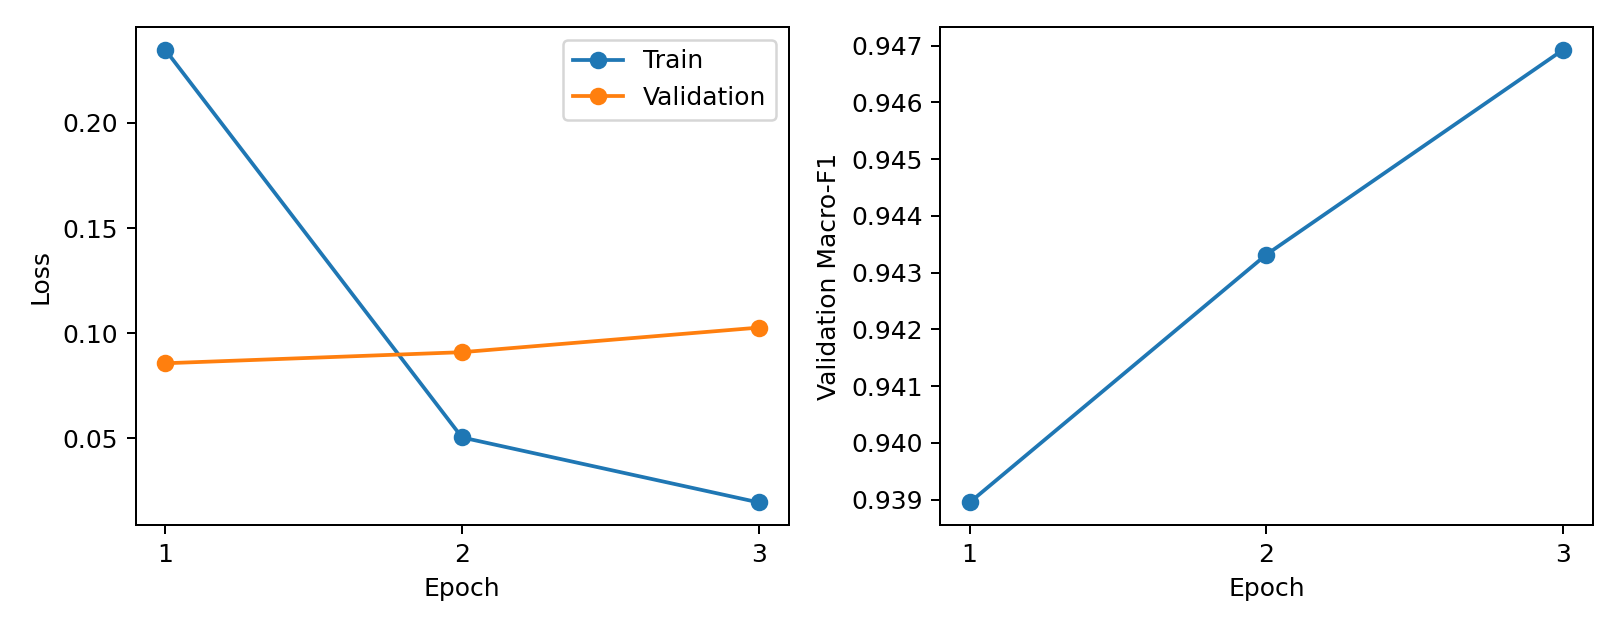
\includegraphics[width=.95\linewidth]{bert_training.png}
\caption{训练、验证损失与验证 Macro-F1。}
\end{figure}
训练 loss 持续下降，说明模型越来越适应训练数据。验证 loss 有所上升，但验证 Macro-F1 也有所提高。loss 还受预测概率影响，而 Macro-F1 看的是最终分对或分错的类别，所以二者不一定同时变化。

代码按验证 Macro-F1 选模型，因此最终使用第 3 轮。测试集 Accuracy 为 98.44\%，Macro-F1 为 96.62\%，1152 篇中分错 18 篇。
\begin{table}[H]\centering
\begin{tabular}{lrrr}\hline\hline
类别 & 正确篇数 / 总数 & Recall & F1\\\hline
business & 138 / 143 & 96.50\% & 95.17\%\\
politics & 137 / 145 & 94.48\% & 95.14\%\\
sports & 859 / 864 & 99.42\% & 99.54\%\\\hline\hline
\end{tabular}
\caption{BERT 的分类别结果。}
\end{table}
\begin{figure}[H]\centering
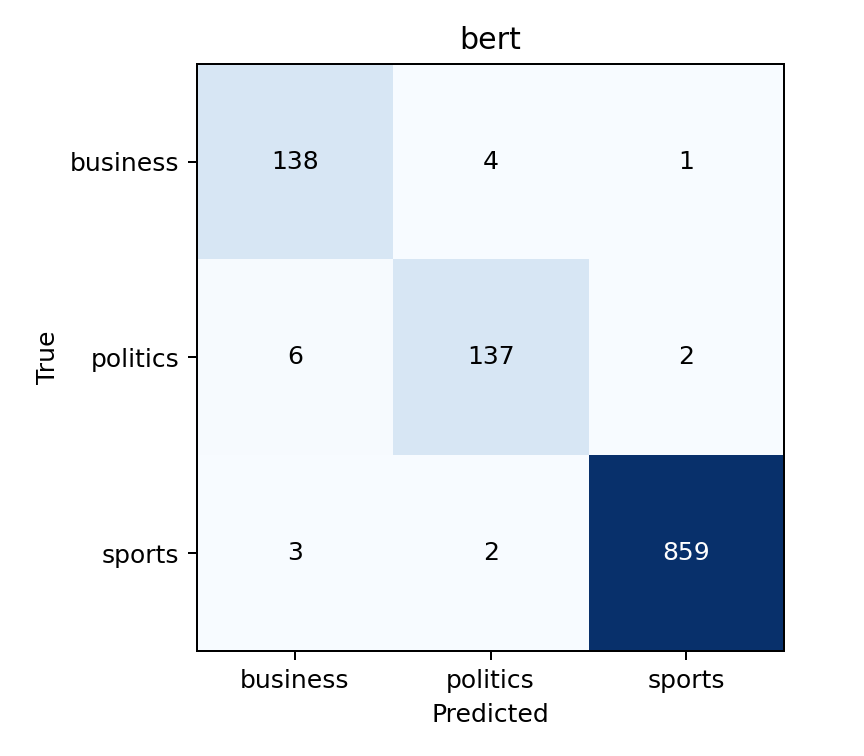
\includegraphics[width=.58\linewidth]{bert_confusion.png}
\caption{BERT 测试集混淆矩阵。}
\end{figure}

\subsection{分析：BERT 为什么没有超过词袋}
BERT 的测试 Macro-F1 为 96.62\%，排第三。它比 Binary 低约 0.57 个百分点，比词频低约 1.03 个百分点。

我认为可能与输入范围和训练条件有关。测试新闻的中位长度为 683 个词，而 BERT 最多只能读取前 62 个正文子词，容易丢失后文的主题信息；词袋则利用全文词频，而关键词本身就能为新闻主题分类提供较强的线索。此外，BERT 仅在 9215 篇训练新闻上微调 3 轮，没有充分调整超参数。从类别表现看，BERT 对商业和政治新闻的区分弱于体育新闻，这也拉低了对各类别等权计算的 Macro-F1。

\subsection{扩展实验：限制词袋的输入范围}
为了进一步观察输入范围的影响，补充一个简单对照：按 BERT 分词器前 62 个正文 WordPiece 的字符位置截取原文，让 Binary 和词频也只使用这段开头文本。训练、验证和测试集都采用相同处理方式，并重新从截短后的训练文本建立词表、训练分类器；$C$ 沿用主实验选定的 0.1，不根据测试集重新调参。词袋仍使用自己的分词规则。

\begin{table}[H]\centering
\begin{tabular}{llrr}\hline\hline
方法 & 输入范围 & 测试 Accuracy & 测试 Macro-F1\\\hline
Binary & 全文 & 98.87\% & 97.18\%\\
Binary & 对齐 BERT 的开头范围 & 96.01\% & 91.76\%\\
词频 & 全文 & 99.05\% & 97.65\%\\
词频 & 对齐 BERT 的开头范围 & 96.44\% & 92.33\%\\
BERT & 64 个位置，含特殊符号 & 98.44\% & 96.62\%\\\hline\hline
\end{tabular}
\caption{扩展实验：全文与短输入的比较，BERT 采用主实验结果。}
\end{table}
词频模型的 Macro-F1 从 97.65\% 降到 92.33\%，下降约 5.32 个百分点，Binary 也出现明显下降。这说明全文确实为词袋提供了有用信息。限制到相同开头范围后，BERT 比短输入词频高约 4.29 个百分点，说明它在短文本条件下仍有较好的分类能力。

\section{结果比较}
\subsection{结果汇总}
\begin{table}[H]\centering
\begin{tabular}{llrr}\hline\hline
任务 & 方法 & Accuracy & Macro-F1\\\hline
Task 1 & Binary BoW & 98.87\% & 97.18\%\\
Task 1 & Word Frequency & 99.05\% & 97.65\%\\
Task 2 & GloVe 100d & 98.35\% & 96.19\%\\
Task 2 & Word2Vec AG & 97.14\% & 93.07\%\\
Task 2 & Word2Vec NYT & 98.00\% & 95.06\%\\
Task 3 & BERT & 98.44\% & 96.62\%\\\hline\hline
\end{tabular}
\caption{六组实验使用同一测试集的结果。}
\end{table}
\begin{figure}[H]\centering
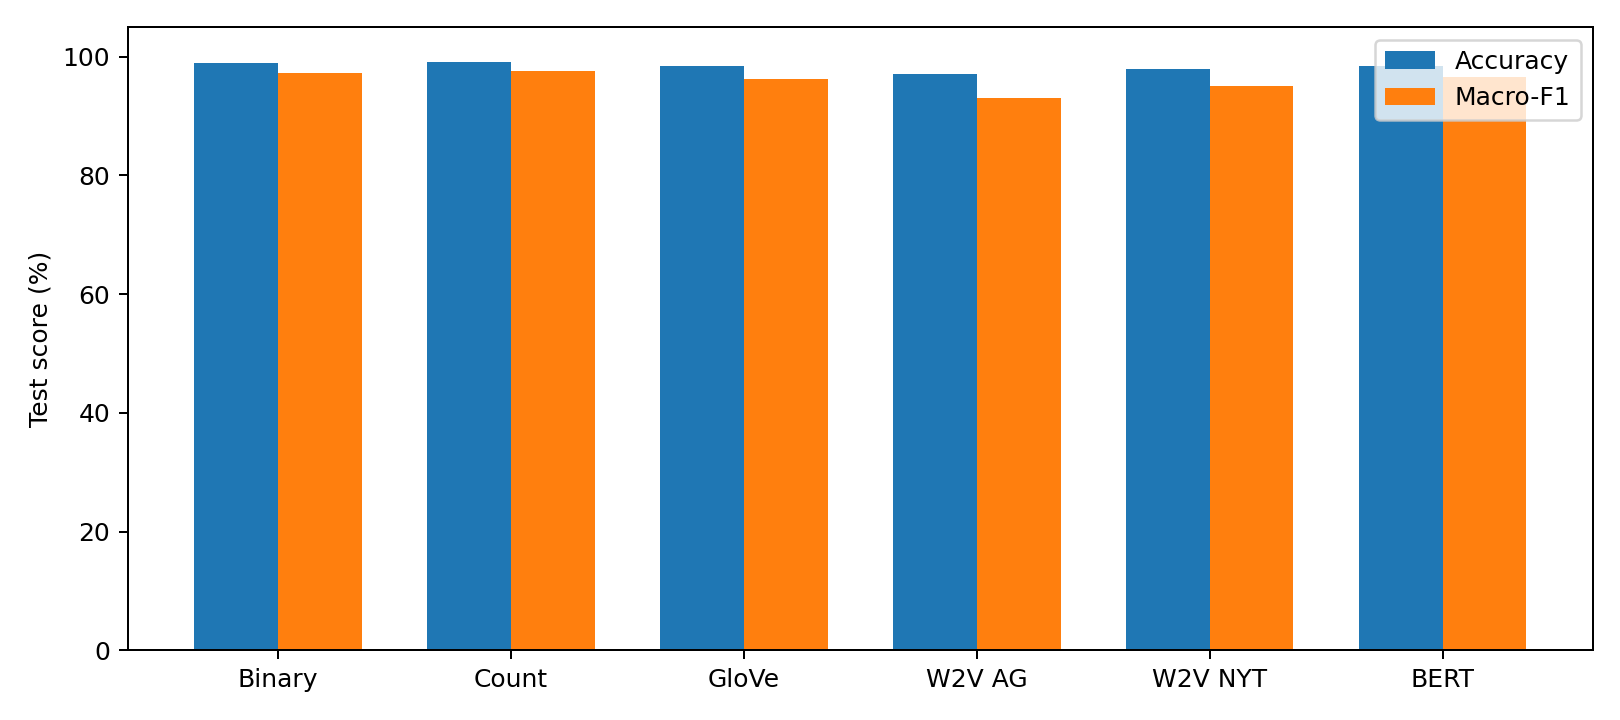
\includegraphics[width=.95\linewidth]{metrics.png}
\caption{Accuracy 与 Macro-F1 的总体比较。}
\end{figure}
本次词频模型最高，Binary 次之。BERT 的两个指标均高于三组平均词向量，但没有超过两种词袋。三组词向量中 GloVe 最好，NYT Word2Vec 高于 AG Word2Vec。




\subsection{对结果的理解}
\textbf{词袋为什么表现很好？}新闻类别常有明显的关键词。词袋虽然不懂词序和语义，却能直接保存这些关键词是否出现、出现多少次，再用分类器学到它们与类别的关系。在这种主题分类任务里，简单方法也可以取得很好的效果。

\textbf{词向量为什么没有明显超过词袋？}100 维表示更紧凑，也能表示词之间的相似性，但普通平均会混合全文信息。主题词、背景词都参与平均，某个特别重要的词可能不再突出。词向量学得好，并不代表平均出来的文档向量一定最适合分类。

\textbf{为什么 BERT 没有最高？}BERT 可以结合上下文理解输入，但这次只看前 64 个位置。很多 NYT 新闻较长，后面才出现关键身份或主题信息，这可能限制了bert的模型能力。

\section{实验总结}
本次完成了从数据划分、文本表示、模型训练到结果评价的完整流程。Task 1 帮助我理解词表、稀疏矩阵与词频；Task 2 把单词表示和文档表示区分开；Task 3 则把表示模型和分类层一起更新，并需要注意批处理、训练模式和模型保存。

分析中我发现，单看总分容易得出过于简单的结论。词频并非每篇都优于 Binary，NYT Word2Vec 并非每篇都优于 AG，BERT 也会受到输入范围限制。更好的做法是把具体结果与方法保留、丢失的信息对应起来。


\end{document}
